% use the "wcp" class option for workshop and conference proceedings
\documentclass[pmlr,twocolumn,10pt]{jmlr} % W&CP article

% Source of the final version. Numbers between double braces come from
% ../numbers/numbers.json (each with the script and CSV that produced it);
% gerar_tex_final.py fills them in and writes ml4h_final.tex. Do not edit the
% generated .tex. Figures: ../analysis/ml4h_figuras_finais.py, drawn at print size.

% ML4H 2026 template: the track must be set before the \iffinal block.
\mlhtrack{findings}

\newif\iffinal
\finaltrue  % final version after acceptance

\iffinal
    \ifmlhneedspmlr
      \jmlrvolume{XXX}
      \jmlryear{2026}
    \fi
    \ifmlhfindings \jmlrproceedings{}{ML4H 2026 - Findings Track}\fi
    \ifmlhdemo     \jmlrproceedings{}{ML4H 2026 - Demo Track}\fi
    \jmlrworkshop{Machine Learning for Health (ML4H) 2026}
\else
    \jmlrproceedings{}{Submitted to ML4H 2026: \mlhtrackname}
    \jmlrworkshop{Machine Learning for Health (ML4H) 2026}
\fi

% amsmath, amssymb, natbib, graphicx, url, algorithm2e, xcolor and hyperref
% are loaded by the class.
\urlstyle{same}
\usepackage{booktabs}
\usepackage{array}
\newcolumntype{L}[1]{>{\raggedright\arraybackslash}p{#1}}
\setlength{\tabcolsep}{4pt}
% Floats close to the text that cites them.
\setcounter{dbltopnumber}{2}
\renewcommand{\dbltopfraction}{0.9}
\renewcommand{\topfraction}{0.9}
\renewcommand{\textfraction}{0.08}
\renewcommand{\dblfloatpagefraction}{0.8}
\renewcommand{\floatpagefraction}{0.8}

\definecolor{boxbg}{HTML}{F3F2EE}
% \ci{1.08 [1.05, 1.12]}: estimate over its interval, for narrow table cells.
\newcommand{\ci}[1]{\cisplit#1\relax}
\def\cisplit#1 [#2]\relax{\begin{tabular}[t]{@{}r@{}}#1\\{\footnotesize[#2]}\end{tabular}}
\newcommand{\runin}[1]{\noindent\textbf{#1.}\ }
\newcommand{\keyfindings}[1]{\par\smallskip\noindent\colorbox{boxbg}{\parbox{\dimexpr\linewidth-2\fboxsep\relax}{\small #1}}\par\smallskip}

\hypersetup{pdftitle={Auditing Identity Noise and Linkage Degradation at National Scale}}

\title[Auditing Linkage Degradation at National Scale]{Auditing Identity Noise and Linkage Degradation at National Scale: From Bias Measurement to Downstream Clinical Distortion}

% Author list: must match OpenReview exactly (names, order).
\author{%
 \Name{Jo\~ao Luis Reis Freitas\nametag{\textsuperscript{a}}},
 \Name{Leonardo Dexheimer {da Silva}\nametag{\textsuperscript{a}}},\\
 \Name{Felipe Matias Berg\nametag{\textsuperscript{b,c}}},
 \Name{Nelson Wolosker\nametag{\textsuperscript{a,b}}}\\
 \addr \textsuperscript{a}Faculdade de Medicina, Universidade de S\~ao Paulo, Avenida Doutor Arnaldo 455, 01246-903, S\~ao Paulo, SP, Brazil\\
 \addr \textsuperscript{b}Hospital Israelita Albert Einstein, Avenida Albert Einstein 627, 05652-900, S\~ao Paulo, SP, Brazil\\
 \addr \textsuperscript{c}Department of Radiology, Case Western Reserve University, 10900 Euclid Avenue, Cleveland, OH 44106, USA
}

\begin{document}

\maketitle

\begin{abstract}
Machine learning on health records assumes that each patient's history has been
stitched together correctly. Where no universal patient identifier exists,
records are linked on demographic fields such as birth date, sex and place, and the errors this introduces
are rarely measured. We audit record linkage across Brazil's public health system (outpatient,
inpatient and mortality systems, 2008--2025, with 3.9 billion outpatient
records, plus the national hospital cancer registry) and follow the measured errors into a
clinical estimate and a trained model. With the health-card number hidden and
used only as ground truth, the linkage cascade reaches 94.6\% recall and
96.0\% precision in a candidate pool the size of a disease cohort, but
36.7\% and 36.8\% across a whole state. Recall is 12.0 points lower where race
is not recorded (6.0 [4.9, 7.2] after adjusting for year and state). In 2{,}684
children with nephroblastoma, losing links at the measured rates moves 5-year
survival from 80.5\% to at most 81.7\%, omitting the mortality
sources moves it to 89.1\%, and deaths that no source records leave the
reference between 77.5\% and 82.7\%. In a breast-cancer
survival model (209,387 patients), the source that labels death moves the stage
IV hazard ratio from 2.52 to 8.07 and changes calibration
by race. Which sources are linked shapes what a model learns more than how many
links are lost.
\end{abstract}

\begin{keywords}
record linkage, data quality auditing, label noise, algorithmic fairness,
administrative health data, survival analysis
\end{keywords}

\paragraph*{Data and Code Availability} All data are open microdata published
by the Brazilian government and downloadable without registration: the
outpatient (SIA), inpatient (SIH) and mortality (SIM) systems from DATASUS
\citep{datasus} (\url{https://datasus.saude.gov.br/transferencia-de-arquivos/}),
and the National Cancer Institute's hospital cancer registry (RHC)
(\url{https://irhc.inca.gov.br/RHCNet/visualizaTabNetExterno.action}; choosing
the case base and the years returns the yearly record-level files). The analysis
scripts, the aggregate output tables behind every number and figure, and a map
from each number to its script and table are available at
\url{https://github.com/jolurf/ml4h2026-linkage-audit}. No record-level data are released.

\paragraph*{Institutional Review Board (IRB)} Brazilian research-ethics norms
exempt research that uses only public-access information from ethics-committee
registration (Resolu\c{c}\~ao CNS 510/2016, Art.~1, sole paragraph, items II
and III). The files contain record-level date of birth, sex and municipality,
and the health-card number is released encrypted: the data are pseudonymised,
not anonymous. We attempted no re-identification, linked no source outside
these files, and report aggregates only.

% =====================================================================
\section{Introduction}
\label{sec:intro}

\begin{figure*}[t]
\floatconts
  {fig:overview}
  {\caption{Overview. (a) A patient's records sit in four national systems, and
  only the outpatient file carries the health-card number; everything else is
  attached by demographic fields (birth date or age, sex, place). (b) The study in
  three steps, with the experiments (E1--E5, Table~\ref{tab:experiments}) and the
  metric of each. FNR: false-negative rate; HR: hazard ratio.}}
  {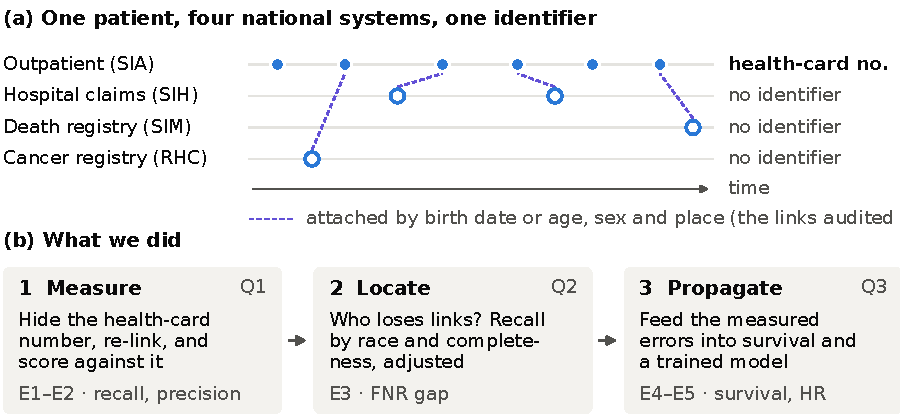
\includegraphics[width=\linewidth]{figures/fig1_overview.pdf}}
\end{figure*}


Clinical machine learning on administrative data treats each patient's
trajectory as given. Where there is no universal patient identifier --- the
situation of most of the world's population --- that trajectory is assembled by
record linkage on birth date, sex and place, and every model trained on it
inherits the linkage errors: a missed link deletes an event, and a false link
attaches someone else's (Figure~\ref{fig:overview}a). These errors are rarely
measured. Work on linkage bias has mostly studied systems where names are
available \citep{harron2014,doidge2019}, and work on algorithmic fairness
usually takes the assembled record as given \citep{obermeyer2019,hardt2016}.

Brazil's Unified Health System (SUS) serves more than 200 million people and
publishes its records as open microdata. Only the outpatient file carries a
patient identifier, the encrypted national health-card number (CNS); hospital
claims, the death registry and the cancer registry do not. Every longitudinal
study built on these files therefore depends on demographic linkage. We use the
places where the identifier \emph{does} exist to measure how well that linkage
works, and then follow the measured errors downstream. We ask three questions
(Figure~\ref{fig:overview}b):
\begin{itemize}
\item[\textbf{Q1}] How accurate is demographic linkage, judged against an
identifier it did not use?
\item[\textbf{Q2}] Whom does it fail?
\item[\textbf{Q3}] How much do linkage errors, and the choice of which sources
to link, change a clinical estimate and a trained model?
\end{itemize}

This is a measurement paper. Its contributions are:
\textbf{(1)} a national audit of the identifier and a validation of the linkage
cascade with the identifier hidden, reporting recall and precision per tier and
showing that both depend on the size of the candidate pool (E1--E2);
\textbf{(2)} an analysis of who loses links, as a difference in false-negative
rates between groups: recall is lower where race is not recorded, and the gap
persists after adjustment (E3);
\textbf{(3)} an error budget for a paediatric cancer cohort that separates three
sources of error and measures the effect of each on survival (E4);
\textbf{(4)} a survival model trained under three death labels, showing that the
label source, which is a linkage decision, changes the coefficients and the
calibration by race (E5).

\keyfindings{\textbf{Key findings.}
\textbf{(i)} Demographic keys identify patients only inside a pool the size of a
disease cohort: recall 94.6\% and precision 96.0\% there; both fall to
36.7--36.8\% across a whole state.
\textbf{(ii)} Links are lost most where registration is incomplete: recall is
12.0 points lower where race is missing.
\textbf{(iii)} Losing existing links at the measured rates moves 5-year survival
little (80.5\% to at most 81.7\%); leaving out the mortality
sources moves it to 89.1\%; and the source that labels death moves a
model's stage IV hazard ratio from 2.52 to 8.07.}

% =====================================================================
\section{Related Work}
\label{sec:related}

CIDACS-RL \citep{barbosa2020} links Brazilian birth and welfare records with
name-based probabilistic matching at national scale and reports link accuracy.
\citet{harron2014} and \citet{doidge2019} show that linkage error biases
epidemiological estimates and propose ways to characterise it, in linked cohorts
where names are available. GUILD \citep{gilbert2018} specifies what
linkage-quality information should be reported. Fellegi--Sunter
\citep{fellegi1969} and its extensions \citep{winkler2006} give the
probabilistic framework that we use as an audit instrument. We differ in the
identifier, the grain and the endpoint (Table~\ref{tab:prior}): no names are
available, the only identifier is encrypted and absent from three of the four
systems, and we follow the measured error into a survival estimate and a trained
model.

\begin{table}[t]
\floatconts
  {tab:prior}
  {\caption{Relation to prior linkage-quality work.}}
  {\small
  \begin{tabular}{@{}L{0.22\linewidth}L{0.19\linewidth}L{0.5\linewidth}@{}}
  \toprule
  Work & Identifier & Endpoint \\
  \midrule
  CIDACS-RL & names & link accuracy \\
  Harron, Doidge & names & bias in estimates \\
  GUILD & any & reporting standard \\
  \textbf{This work} & \textbf{none} (demo\-graphics) & \textbf{link accuracy, bias by group, survival and a trained model} \\
  \bottomrule
  \end{tabular}}
\end{table}

% =====================================================================
\section{Data and Linkage}
\label{sec:data}

\runin{Sources} Table~\ref{tab:sources} lists the four systems. The outpatient
system SIA is distributed as sub-files: BI (outpatient bulletins) is the only one
with the CNS \emph{and} an exact birth date on the same row; AQ and AR
(chemotherapy and radiotherapy authorisations) carry the CNS but only age. The
inpatient system SIH, the death registry SIM and the cancer registry RHC carry no
CNS. Throughout, \emph{registry} means the cancer registry; the death registry is
called SIM. A glossary is in Appendix~\ref{app:glossary}.

\begin{table}[t]
\floatconts
  {tab:sources}
  {\caption{The four systems. ID: encrypted health-card number (CNS).}}
  {\small
  \begin{tabular}{@{}L{0.36\linewidth}llc@{}}
  \toprule
  System & One row is & Birth date & ID \\
  \midrule
  SIA-BI (outpatient) & a visit & exact & yes \\
  SIA-AQ/AR (oncology) & a treatment & age & yes \\
  SIH (hospital) & an admission & exact & no \\
  SIM (deaths) & a death & exact & no \\
  RHC (cancer) & a tumour & age & no \\
  \bottomrule
  \end{tabular}}
\end{table}

\runin{Linkage} A patient is a CNS plus its canonical birth date in BI. Three
links attach everything else (Figure~\ref{fig:links}, Table~\ref{tab:keys}).
Hospital claims are attached by a cascade that stops at the first rule that finds
a candidate (R1--R4). Deaths come either from a death flag on the patient's own
records (C1, no link) or from SIM (C2). The cancer registry records age, not birth
date, so it is attached by facility and sex with nearby diagnosis dates. We call
the whole linkage of SUS records --- the cascade, C1 and C2 --- the
\emph{pipeline}.

\begin{table}[t]
\floatconts
  {tab:keys}
  {\caption{The links and their keys. Ties within a rule go to the smallest
  identifier (cascade) or the closest diagnosis date and then the birth year
  estimated from age (registry).}}
  {\small
  \begin{tabular}{@{}lL{0.78\linewidth}@{}}
  \toprule
  Link & Key \\
  \midrule
  R1 & birth date + facility \\
  R2 & birth date + postal code \\
  R3 & birth date + sex + municipality of residence \\
  R4 & birth date + sex + municipality of the facility \\
  C2 & birth date + sex + municipality at death, and a diagnosis code of the patient on the death certificate \\
  Registry & facility (else municipality) + sex, diagnosis dates $\leq$ 75 days apart \\
  \bottomrule
  \end{tabular}}
\end{table}

\begin{figure*}[t]
\floatconts
  {fig:links}
  {\caption{The links and the evidence available for each. Above each arrow, the
  link; in italics, how it is validated and in which experiment. Only the link
  between the two outpatient files has the identifier on both sides; every link
  the clinical estimates depend on is validated indirectly.}}
  {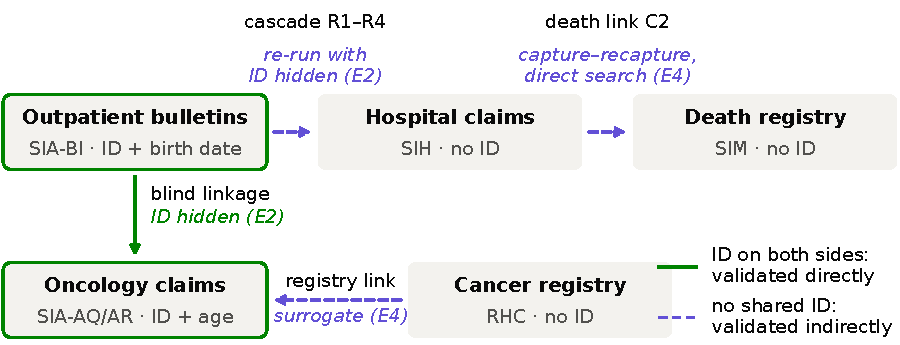
\includegraphics[width=\linewidth]{figures/fig2_sources_links.pdf}}
\end{figure*}

% =====================================================================
\section{Evaluation Design}
\label{sec:design}

\runin{What can be validated, and how} A link can be scored directly only where
the CNS exists on both sides, that is, inside the outpatient files. We use this
twice, always hiding the CNS from the linkage and using it only to score the
result. First, a \emph{blind linkage} of BI with AQ (the \emph{file pair}). Second,
the production cascade re-run inside BI: one record per patient is held out as
the query, the other records are the candidates, the production tie-break picks
the link, and the hidden CNS says whether it is right. Links without an
identifier on either side (hospital claims, deaths, cancer registry) are
validated indirectly: by a surrogate test of the registry link inside SIA, by the
registry's independent death record, by searching SIM directly, and by
capture--recapture between two death lists.

\runin{Metrics} Table~\ref{tab:metrics} lists every metric and where it is used,
and Table~\ref{tab:linkev} what is known about each link. \runin{Experiments}
Table~\ref{tab:experiments} lists the five experiments.

\begin{table}[t]
\floatconts
  {tab:linkev}
  {\caption{What is known about each link ($\leq$: upper bound). The file pair shares
  only municipality and sex, so it measures whether true pairs survive blocking and
  classification, not which candidate is right.}}
  {\small
  \begin{tabular}{@{}L{0.22\linewidth}L{0.31\linewidth}rr@{}}
  \toprule
  Link & Checked against & Recall & Precision \\
  \midrule
  File pair & hidden CNS & 97.32\% & --- \\
  Cascade & hidden CNS, inside BI & 94.6\% & 96.0\% \\
  Registry link & CNS, surrogate in SIA & $\leq$86.7\% & $\leq$93.6\% \\
  SIM link (C2) & direct search of SIM & \multicolumn{2}{r}{loses $\geq$27\%} \\
  \bottomrule
  \end{tabular}}
\end{table}

\begin{table}[t]
\floatconts
  {tab:metrics}
  {\caption{Metrics.}}
  {\small
  \begin{tabular}{@{}L{0.27\linewidth}L{0.5\linewidth}l@{}}
  \toprule
  Metric & Definition & Used in \\
  \midrule
  Recall & true pairs linked correctly / true pairs & E2, E3 \\
  Precision & correct links / links made & E2 \\
  FNR gap & difference in $1-$recall between groups (equal opportunity, \citealp{hardt2016}) & E3 \\
  Validity & share of records whose CNS passes the composite check & E1 \\
  Cadastral entropy & entropy of the identities recorded under one CNS & E1 \\
  Candidate-pair score & Fellegi--Sunter weight of a candidate pair & E1 \\
  5-year OS; stage IV HR & Kaplan--Meier survival; univariate Cox hazard ratio & E4 \\
  HR; C-index & Cox coefficients; discrimination & E5 \\
  Calibration & predicted $-$ observed 5-year risk (negative: under-prediction); decile error: its absolute value averaged over deciles & E5 \\
  \bottomrule
  \end{tabular}}
\end{table}

\begin{table*}[t]
\floatconts
  {tab:experiments}
  {\caption{The five experiments. ``Compared with'' is the reference each result
  is scored against.}}
  {\small
  \begin{tabular}{@{}lL{0.28\linewidth}L{0.21\linewidth}L{0.16\linewidth}L{0.15\linewidth}l@{}}
  \toprule
  & Question & Data & Compared with & Metric & Section \\
  \midrule
  E1 & Q1: how reliable is the identifier? & all BI records, 2008--2025; file pair for the score & check digit; chance & validity, entropy, score & \ref{sec:e1} \\
  E2 & Q1: does the linkage find the right patient? & BI$\times$AQ; cascade in BI, 3 states & hidden CNS & recall, precision & \ref{sec:e2} \\
  E3 & Q2: who loses links? & BI$\times$AQ & hidden CNS, adjusted & FNR gap & \ref{sec:e3} \\
  E4 & Q3: how much does survival move? & nephroblastoma, 2{,}684 children & reference cohort & 5-year OS, HR & \ref{sec:e4} \\
  E5 & Q3: does the death label change a model? & breast cancer, 209,387 patients & union label, test set & HR, calibration & \ref{sec:e5} \\
  \bottomrule
  \end{tabular}}
\end{table*}

% =====================================================================
\section{Results}
\label{sec:results}

\subsection{E1: The Identifier Is Usable but Not Clean}
\label{sec:e1}

\begin{figure}[t]
\floatconts
  {fig:cascade}
  {\caption{The cascade R1$\to$R3$\to$R4 with the CNS hidden (3 states). Each
  held-out record ends in a correct link (its share is the recall), a wrong link,
  or no link. Details by rule and state: Appendix~\ref{app:cascade}.}}
  {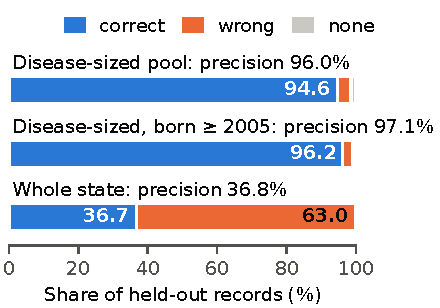
\includegraphics[width=\linewidth]{figures/fig3_cascade_pools.pdf}}
\end{figure}


\runin{Setup} A CNS is reliable if it is well-formed, not a repeated-character
placeholder, associated with at most three birth dates, and passes the official
check digit. \emph{Cadastral entropy} is computed per CNS: the Shannon entropy of
the distinct (birth date, sex, municipality) identities recorded under it, with
the Miller--Madow correction \citep{miller1955}; it is zero when a number always
carries one identity. The \emph{candidate-pair score} is the Fellegi--Sunter
weight $\sum_f \log_2(m_f/u_f)$ over the fields a candidate pair shares, where
$u_f$ is the agreement rate among different people and $m_f$ among records of
the same person.

\runin{Results} 87.17\% of 3.9 billion outpatient (BI) records carry
a reliable identifier. Reliability improves with calendar year (58.3\% unreliable in 2008,
5.8\% in 2024) and differs by race: standardised to the overall year
distribution, unreliability is 13.5\% for Black, 11.5\%
for mixed-race and 9.6\% for White records, so year does not
explain the difference. Of 235.6 million distinct well-formed numbers, 19.81\%
carry more than one recorded identity (mean entropy 0.176 bits); of these, 59.6\%
differ only in municipality, consistent with moving house, and 40.4\% in
birth date or sex, which is contamination. In the other direction, 50.96\% of
(birth date, sex, municipality) triplets appear under more than one CNS, against
38.5\% expected by chance alone. On the file pair, the candidate-pair
score separates true from false matches: its highest bucket has a true-match
rate 177 times that of its lowest (Appendix~\ref{app:audit}).

\runin{Takeaway} One number often carries more than one identity, and one
identity is often shared by different people: neither the identifier nor the
demographics alone define a patient.

\subsection{E2: Linkage Works Inside a Disease Pool, Not Across a Population}
\label{sec:e2}

\begin{figure*}[t]
\floatconts
  {fig:race}
  {\caption{(a) Recall with the CNS hidden, by recorded race/colour (95\% CI).
  (b) The recall gap where race is missing, crude and adjusted. Intervals are
  cluster-robust by state (adjusted) and bootstrapped over facilities (within
  facility and year).}}
  {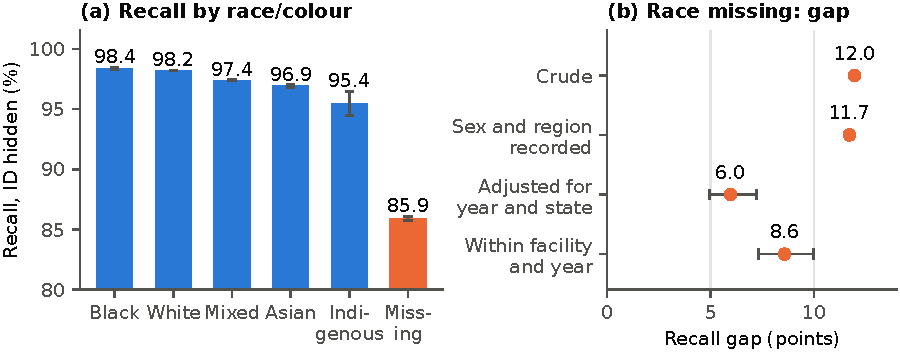
\includegraphics[width=\linewidth]{figures/fig4_race_recall.pdf}}
\end{figure*}


\runin{Setup} The blind BI$\times$AQ linkage blocks on municipality and then
classifies on sex. AQ has no birth date, so it cannot test R1--R4; for that, we
re-ran the cascade R1$\to$R3$\to$R4 inside BI in three states (Acre, Sergipe
and Mato Grosso do Sul), with three
candidate pools: a \emph{disease-sized} pool (1\% of each state's patients,
drawn by a salted hash of the CNS, with all their records), the same restricted
to patients born from 2005 (paediatric-like), and the whole state. The pipeline
uses disease-sized pools, because it filters diagnoses on both sides before
linking. R2 cannot be tested: BI has no postal code.

\runin{Results} The blind linkage recovers 97.32\% of 2{,}783{,}627 true pairs;
almost all of the loss happens at blocking. Because the file pair shares only
municipality and sex, this is a recall: it says whether true pairs survive
blocking and classification, not which candidate is right. Precision is measured
on the cascade. The cascade results are in
Figure~\ref{fig:cascade}. In a disease-sized pool, recall is 94.6\% and
precision 96.0\%. R1 alone links 81.1\% correctly; of the
9,585 queries it leaves unlinked, R3 and R4 link 85.1\% correctly,
while R1's own wrong links are not revisited. Precision per rule is
96.4\% (R1), 94.7\% (R3) and 71.2\% (R4). Against a
whole state, both recall and precision fall to about 36.8\%.

\runin{Takeaway} Demographic keys identify people only in the small pool that a
disease filter leaves; at population scale most agreements are coincidences. So
chance agreement must be measured in the pool actually compared. The same holds
for Fellegi--Sunter parameters: nationally, the joint $u$ of birth date + sex +
municipality is 1.02$\times$ the product of the single-field values,
so independence nearly holds, whereas in the nephroblastoma pool it is
7.7--30.4$\times$ (Appendix~\ref{app:fs}).

\subsection{E3: Links Are Lost Where Race Is Not Recorded}
\label{sec:e3}

\begin{figure}[t]
\floatconts
  {fig:budget}
  {\caption{The 474 deaths of the nephroblastoma cohort within five
  years, by the record that holds them, and the link each rests on. Blue: also
  recorded by the cancer registry. Orange: the 95 deaths that a linkage
  cascade could lose (no registry confirmation). The registry confirms deaths
  that rest on a hospital claim as often as deaths on records with the CNS
  (68.9\% and 67.5\%).}}
  {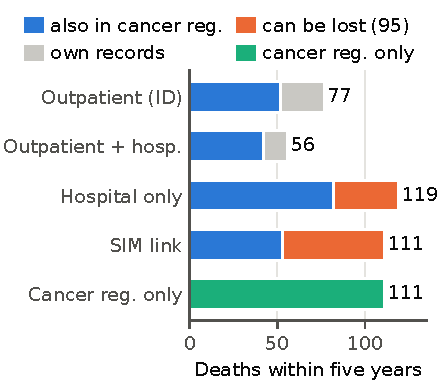
\includegraphics[width=\linewidth]{figures/fig5_death_budget.pdf}}
\end{figure}


\runin{Setup} On the file pair, we compare recall across recorded race/colour
groups and where race is missing. Because missing race travels with other gaps,
we estimate the gap three ways: among records with sex and region present; with a
logistic model with year and state fixed effects (g-computation, standard errors
clustered by state); and within the same facility and year (Mantel--Haenszel
\citep{mantel1959} over facility $\times$ year strata, bootstrap over
facilities). All intervals account for clustering, by bootstrap over
municipalities, facilities or states or by standard errors clustered by state;
none resamples records.

\runin{Results} Recall is 85.9\% where race is missing against
97.9\% where it is recorded; recorded groups range from
95.4\% (Indigenous) to 98.4\% (Black)
(Figure~\ref{fig:race}). The gap is 11.7 points among records with sex and
region present, 6.0 [4.9, 7.2] points after adjusting for year and state, and
8.6 [7.3, 10.0] points within the same facility and year. Between recorded groups, FNR
differences are small but remain after clustering: Black/mixed vs.\ White
0.67 [0.49, 0.85] points and North/Northeast vs.\ South/Southeast 2.30 [1.94, 2.66] points
(bootstrap over municipalities; over states, 0.67 [0.22, 1.20] and 2.30 [1.51, 3.42]).

\runin{Takeaway} Missing race marks records that are harder to link. This is
consistent with a pathway through registration completeness, but we fit no
causal model, and we read the association descriptively.

\subsection{E4: What Moves a Survival Estimate}
\label{sec:e4}

\begin{figure*}[t]
\floatconts
  {fig:scenarios}
  {\caption{5-year OS (a) and stage IV HR (b) of the nephroblastoma cohort under
  each error scenario, grouped by the source of error. Grey band: 95\% sampling
  CI of the reference; dashed line: the reference. Random scenarios show the
  median over 1{,}000 draws. The upper-bound false-link scenario treats every
  ambiguous SIM death as false. Full table: Appendix~\ref{app:scenarios}.}}
  {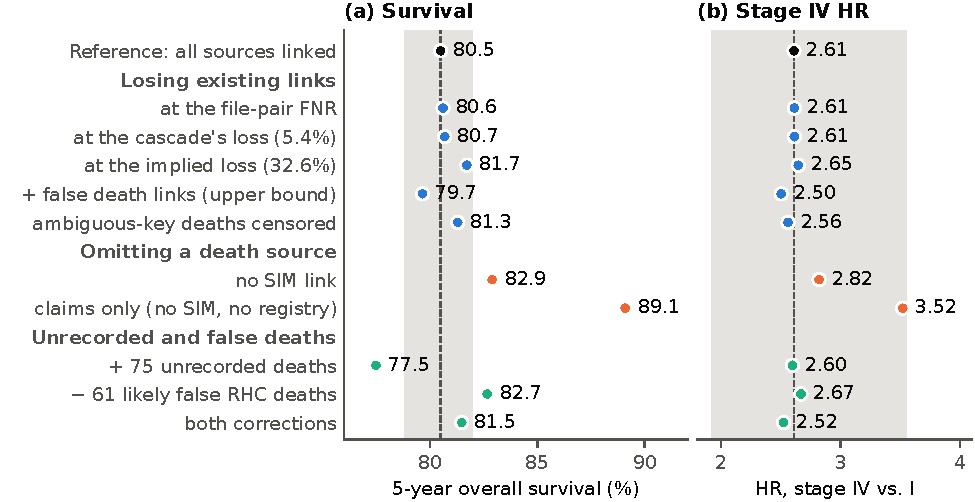
\includegraphics[width=\linewidth]{figures/fig6_scenarios.pdf}}
\end{figure*}


\runin{Setup} We reconstruct a national cohort of children with nephroblastoma
(Wilms tumour, 2008--2023; 2{,}684 patients, histology confirmed by the cancer
registry) and follow them for five years. The reference records 474
deaths: 5-year overall survival (OS) 80.5\% [78.8, 82.0], univariate
stage IV hazard ratio (HR) 2.61 [1.92, 3.55]. Every death rests on some link,
and the links differ in what can be measured (Figure~\ref{fig:budget}): the
95 deaths that the audited cascades can lose are 58 through the
SIM link and 37 through a hospital claim, in both cases without
confirmation by the cancer registry. The whole cohort rests on the registry link,
which, tested against the CNS inside SIA, has 93.6\% precision and
86.7\% recall (upper bounds, Appendix~\ref{app:rhclink}). We then perturb
the reference in three ways:
\begin{itemize}
\item \emph{Losing existing links.} The 95 cascade-dependent death links
are removed at three loss rates, 1{,}000 draws each. (1) The file-pair FNR of the
patient's completeness stratum (how many of sex, race and region are recorded):
a floor for the SIM step, which also needs a matching diagnosis code. (2) The
cascade's loss with the CNS hidden (5.4\%). (3) The loss implied by
capture--recapture: the pipeline records 67\% of the deaths that
capture--recapture estimates, so it misses 32.6\%. We also add false
death links, at most at the rate that treats every ambiguous SIM death as false.
\item \emph{Omitting a death source.} Without the SIM link, and with claims
only: death flags on the patient's own outpatient and hospital records, with no
SIM link and no cancer registry.
\item \emph{Unrecorded and false deaths.} The pipeline and the cancer registry give
two lists of deaths; capture--recapture (Chapman, \citealp{chapman1951})
estimates the deaths neither records. Registry deaths not found in SIM by a
direct search are likely attached to the wrong patient.
\end{itemize}

\runin{Results} Figure~\ref{fig:scenarios} shows every scenario. \emph{Losing
links} moves OS little: to 80.6\% at the measured FNR, 80.7\% at the
cascade's loss and 81.7\% at the loss implied by capture--recapture,
because the registry backs up most of what the SIM link loses. Moving OS by one
point requires losing 26\% of these links; losing all of them moves it
3.9 points. \emph{Omitting a source} moves it a lot: with claims only,
the cohort records 252 deaths and OS rises to 89.1\% (HR
3.52); without the SIM link alone, to 82.9\%. \emph{Unrecorded and
false deaths} move it both ways. Capture--recapture estimates 539
[515, 563] deaths, so about 65
[41, 89] are recorded by neither list; stratified by
stage the estimate is 75, and adding them lowers OS to
77.5\%. Both lists come from hospitals, so a well-registered patient
tends to appear in both, and this dependence makes the estimate too small. False
links push the other way: searching SIM for each registry-only death by date of
death and birth date finds 42 of 111. Our SIM link missed
these; it found 111 others, so it loses at least 27\%
(42 of 153) of the deaths SIM holds for this
cohort. After the search key's own miss rate, about
61 registry-only deaths are not in SIM at all, an upper bound. Removing them raises OS to 82.7\%; doing
both gives 81.5\%. The reference lies inside this bracket, and across
these corrections the stage IV HR stays between 2.52 and
2.67.

The racial gap behaves the same way. White patients have a 5-year OS
5.0 points higher than Black or mixed-race patients (sampling CI
[1.8, 8.2]); under race-differential link loss at the measured ratio the gap is
5.0 [4.7, 5.2], and it narrows as loss grows (Appendix~\ref{app:propagation}), so
linkage error would understate the disparity. Treating race as the missing
variable, complete cases, inverse probability weighting and multiple imputation
give the same HR for White vs.\ Black/mixed-race patients (0.741 [0.610, 0.900], 0.743 [0.610, 0.904] and 0.734 [0.604, 0.891]; Appendix~\ref{app:race}).

\runin{Takeaway} For this estimate, the errors that matter are not the links lost
at the measured rates but the sources left out and the deaths that no source
records.

\subsection{E5: A Trained Survival Model Inherits the Death Label}
\label{sec:e5}

\begin{figure*}[t]
\floatconts
  {fig:model}
  {\caption{Breast-cancer Cox model trained under three death labels. (a, b) HR
  with 95\% CI. (c) Under-prediction of 5-year risk against the union label, test
  set, for the pipeline- and registry-trained models.}}
  {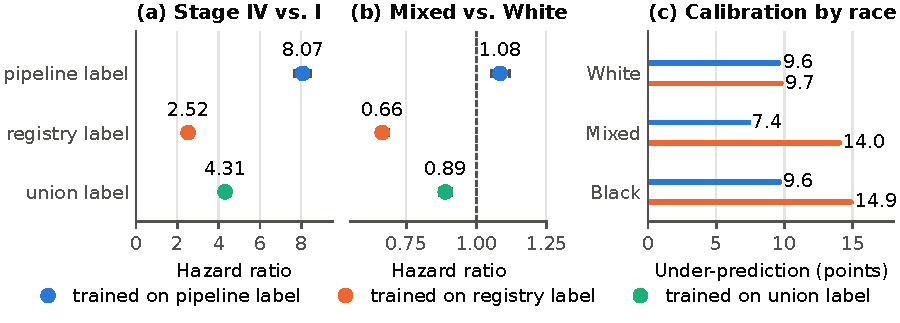
\includegraphics[width=\linewidth]{figures/fig7_model_labels.pdf}}
\end{figure*}


\runin{Setup} We fitted a Cox model (age, stage I--IV, race, year, region, and a
standardised social vulnerability index of the patient's area) to a national breast-cancer cohort linked to the cancer registry
(209,387 patients; 70/30 train/test split), three times, changing only the
source that labels death. The \emph{pipeline} label is a death flag on the
patient's own treatment records (C1; 59\% of its 40,755 deaths)
or a SIM death found by the demographic link (C2); the \emph{registry} label is
the cancer registry's death date (31,281 deaths); the \emph{union} is either
source, earlier date (58,899 deaths). Each model is scored against the
union label on the test set.

\runin{Results} The label changes what the model learns (Figure~\ref{fig:model},
Table~\ref{tab:model}). The stage IV HR ranges from 2.52 to
8.07, and the mixed-race HR changes direction. The union lies between
the others although it has the most deaths in every stage, because its
18,144 registry-only deaths carry no stage gradient
(8.2--9.3\% of patients in every stage). Searched in SIM,
31\% of them are found: deaths our SIM link missed. About
55\% are not in SIM at all, mostly in early stages
(61\% in stage I, 32\% in stage IV). The
figure is indicative, and consistent with registry records attached to the wrong
patient.
The pipeline gradient is steep partly because deaths during treatment (C1)
concentrate in stage IV (Appendix~\ref{app:c50}).

Each model is calibrated to its own label (decile error
0.6--1.1 points). Against the union, the
pipeline-trained model predicts 17.7\% where 26.2\% is
observed and under-predicts all race groups alike, whereas the registry-trained
model under-predicts White patients by 9.7 points but mixed-race
by 14.0 and Black by 14.9. The registry label also
carries region (HR South 0.46 vs.\ 1.04 under the
pipeline label), because the registry's death follow-up differs by hospital; race,
which varies by region, enters the calibration through it. By contrast, losing the
12,344 SIM-link deaths at the measured rate moves the stage IV HR only
from 4.31 to 4.29 (4.28 at the cascade's loss).

\runin{Takeaway} In the model, as in the clinical estimate, which sources label
the outcome matters far more than losing links. The union is the most complete
label, not a gold standard.

\begin{table}[t]
\floatconts
  {tab:model}
  {\caption{Cox model under three death labels (breast cancer). Calibration and
  C-index against the union label, test set.}}
  {\small
  \begin{tabular}{@{}L{0.3\linewidth}rrr@{}}
  \toprule
  & Pipeline & Registry & Union \\
  \midrule
  HR stage IV vs.\ I & 8.07 & 2.52 & 4.31 \\
  HR mixed vs.\ White & \ci{1.08 [1.05, 1.12]} & \ci{0.66 [0.64, 0.69]} & \ci{0.89 [0.87, 0.91]} \\
  Pred./obs.\ 5-year risk & 0.68 & 0.55 & 1.00 \\
  Decile error (points) & 8.7 & 11.6 & 1.1 \\
  C-index & 0.651 & 0.625 & 0.659 \\
  \bottomrule
  \end{tabular}}
\end{table}

% =====================================================================
\section{Discussion}
\label{sec:discussion}

\runin{What the audit shows} Demographic linkage works inside a pool the size of
a disease cohort and fails at population scale; it fails more often where registration is
incomplete, especially where race is missing; and, for a clinical estimate, the
errors that matter are not the links lost at the measured rates but the sources
left out and the deaths that no source records. A model trained on these data
inherits the choice of death source in its coefficients and in its calibration
by race.

\runin{What practitioners can do} Three habits follow. \textbf{Measure chance
agreement in the pool you compare}, not nationally: the same key that is safe in
a disease cohort is useless across a state (E2). \textbf{Report linkage recall by
group}, with missing demographic fields as a group of their own (E3).
\textbf{Treat the outcome sources as part of the model}: state which sources
label the outcome, and bound the events no source records, for example by
capture--recapture between two lists (E4--E5).

\runin{Limitations} The hospital and mortality links have no identifier, so they
are validated only indirectly. The cascade test runs inside BI, with a random
(not the most recent) record held out, in three small states, without R2, and
only for patients with a valid CNS; all of this makes it optimistic for
cross-system links. Capture--recapture assumes independent lists; we bound the
two ways it can fail but cannot remove them. The registry link is validated only
by a surrogate in which the probe belongs to its own reference, so its precision
and recall are upper bounds. Fellegi--Sunter parameters, ambiguity rates and loss
rates are specific to this system and to each disease pool, and must be
re-estimated elsewhere. The racial analyses are descriptive associations, not
causal estimates.

\runin{Next steps} An adjudicated validation of the hospital and mortality links
needs identified records, which require access granted by the Ministry of Health
and ethics-committee approval; we are applying for both. Where links carry a
measured uncertainty, it could enter a temporal graph model as an edge weight or
an edge-dropout probability \citep{rossi2020}.

% =====================================================================
\section{Conclusion}
\label{sec:conclusion}

Auditing a national health system (3.9 billion outpatient records and the
hospital, mortality and cancer registries linked to them), we measured
linkage recall and precision against a hidden identifier, located where recall is
lost, and propagated the measured errors into a survival estimate and a trained
model. Losing links at the measured rates moves the estimates little; omitting a
mortality source, and deaths that no source records, move them substantially; and
a model trained on a single source carries that choice into its calibration by
race.

\acks{[TODO ACKNOWLEDGMENTS AND FUNDING]}

\bibliography{refs}

% =====================================================================
\clearpage
\appendix

\section{Glossary and Data Details}
\label{app:glossary}

\begin{table}[ht]
\floatconts
  {tab:glossary}
  {\caption{Glossary.}}
  {\small
  \begin{tabular}{@{}lL{0.74\linewidth}@{}}
  \toprule
  Term & Meaning \\
  \midrule
  SUS & Unified Health System, Brazil's public health system \\
  CNS & national health-card number; released encrypted \\
  SIA & outpatient information system \\
  \quad BI & individual outpatient bulletins (CNS + birth date) \\
  \quad AQ, AR & chemotherapy and radiotherapy authorisations (CNS + age) \\
  SIH & hospital information system (one row per admission claim) \\
  SIM & mortality information system (one row per death certificate) \\
  RHC & hospital cancer registry of the National Cancer Institute \\
  File pair & the two outpatient sub-files linked blind: BI and AQ \\
  Pipeline & the whole linkage of SUS records: cascade R1--R4, C1 and C2 \\
  Registry & the cancer registry (RHC); the death registry is SIM \\
  R1--R4 & the four rules of the hospital-claim cascade (Table~\ref{tab:keys}) \\
  C1, C2 & death from a flag on the patient's own records; death from SIM by the demographic link \\
  OS; HR & overall survival; hazard ratio \\
  FNR & false-negative rate, $1-$recall \\
  \bottomrule
  \end{tabular}}
\end{table}

\runin{Nephroblastoma cohort} The cancer registry records one row per tumour, and
bilateral disease produces two; the cohort is collapsed to one row per patient
(counting tumour records instead inflates $n$ by 20.6\%).

\runin{Breast-cancer cohort} Patients linked to the cancer registry, stage I--IV,
non-negative follow-up under all three labels and complete covariates
(209,387); administrative end 31 December 2024; split 70/30 stratified by stage
with a fixed seed; no penalisation. Calibration error is the absolute difference
between mean predicted and Kaplan--Meier observed 5-year risk, averaged over
deciles of predicted risk.

\section{National Audit: Definitions and Full Results}
\label{app:audit}

\subsection{CNS Validation and Missingness}
The check-digit implementation agreed with an independent open-source
implementation on 301{,}010 synthetic checks, including 50{,}053 cases of the
branch where the check-digit remainder gives 10 and 1{,}000 single-digit corruptions. Of 3.42 billion records
with a well-formed CNS (about 235.6 million distinct numbers), 99.9999\% pass the
check digit. Missingness is not at random (Table~\ref{tab:mnar}): unreliability
is highest in early years, where race is not recorded, and under one year of age
(37.0\%), when a newborn has often not yet received a personal CNS. Standardised
to the overall distribution of years, CNS unreliability is 13.5\%
(crude 12.7\%) for Black, 11.5\%
(11.0\%) for mixed-race, 9.6\%
(9.3\%) for White and 30.2\% (27.7\%)
where race is not recorded.

\begin{table}[ht]
\floatconts
  {tab:mnar}
  {\caption{Cram\'er's $V$ for CNS reliability by stratum ($n>3.9$ billion
  BI records; all $\chi^2$ $p<10^{-300}$).}}
  {\small
  \begin{tabular}{@{}l@{\hspace{4pt}}r@{\hspace{6pt}}l@{}}
  \toprule
  Dimension & $V$ & Worst-off category \\
  \midrule
  Year of care & 0.324 & 2008 (58.3\%); 2024: 5.8\% \\
  Race/colour & 0.197 & not recorded (27.7\%) \\
  State & 0.135 & Distrito Federal (22.6\%) \\
  Age band & 0.132 & under 1 year (37.0\%) \\
  Facility type & 0.130 & range 0.3\%--53.6\% \\
  Region & 0.061 & Southeast (13.9\%) \\
  Sex & 0.025 & code ``0'' (100\%) \\
  \bottomrule
  \end{tabular}}
\end{table}

\subsection{Collisions and Cadastral Entropy}
\runin{Chance baseline} Under a Poisson null in which each (CNS, triplet) is a
distinct person and birth dates follow the state's distribution within each
municipality $\times$ sex cell, 38.5\% of occupied triplets would hold
more than one CNS, against 50.96\% observed (ratio 1.32). The null
ignores the clustering of birth dates within municipalities and predicts
105.7 million distinct triplets against 90.4 million
observed, so 38.5\% is a lower bound on chance collision: most of the
sharing is different people coinciding.

\runin{Entropy} For a CNS with $N$ records split across $K$ identities with
counts $n_i$, $H=-\sum_i (n_i/N)\log_2(n_i/N)$, and the Miller--Madow
correction adds $(K-1)/(2N\ln 2)$. Mean entropy is 0.176 bits (plug-in
0.154). The share of numbers with more than one identity rises from
14.2\% (2--4 records) to 45.9\% (100 or more), and is nearly
flat across facility-volume deciles (18.3--24.3\%): a patient's own utilisation,
not the facility, drives drift.

\subsection{Candidate-Pair Score}
On BI$\times$AQ pairs blocked by state, only municipality and sex are shared (AQ
has no birth date), so the score takes four values. With $u$ for municipality
measured within state (0.175), matching the blocking, the true-match rate
is monotone in the score, and the highest bucket has a true-match rate 177
times that of the lowest.

\subsection{Recall per Record, Stability and Blocking Precision}
A key is \emph{stable} for a patient if it takes the same value on all of the
patient's BI records: R1 29.66\%, R3 74.81\%, R4 62.02\% (185 million patients
with $\geq 2$ records). This is far stricter than what blocking needs. Per
record --- does a held-out record share the key with any other record of the
same patient? --- recall is 93.7\% for R1, 99.0\% for R3 and 98.3\%
for R4. In the blind BI$\times$AQ linkage, blocking recovers 97.69\% of true
pairs and the classifier (sex) keeps 99.62\% of those; a random pair sharing only
the municipality block is a true match with probability $2.07\times10^{-8}$ (one
in 48.2 million), which is why the classifier stage is needed.

\subsection{Completeness, Recall and FNR}
\label{app:completeness}

\begin{table}[ht]
\floatconts
  {tab:completeness}
  {\caption{Blind-linkage recall (BI$\times$AQ, $n$=2,783,627) by race and by
  completeness score (sex, race and region recorded).}}
  {\small
  \begin{tabular}{@{}lr@{}}
  \toprule
  Stratum & Recall \\
  \midrule
  Completeness 3/3 ($n$=2{,}655{,}529) & 97.9\% \\
  Completeness 2/3 ($n$=127{,}691) & 85.7\% \\
  Completeness 1/3 ($n$=407) & 0.0\% \\
  \midrule
  Race not recorded & 85.9\% \\
  Indigenous ($n$=1{,}581) & 95.4\% \\
  Asian descent & 96.9\% \\
  Mixed (pardo) & 97.4\% \\
  White & 98.2\% \\
  Black & 98.4\% \\
  \bottomrule
  \end{tabular}}
\end{table}

The completeness score includes race, so comparing scores mixes the race question
with missing blocking fields: 99.3\% of the 2/3 stratum lacks race, and the few
records with race but without sex or region cannot be blocked at all. We
therefore estimate the missing-race gap directly: crude 12.0 points;
11.7 among records with sex and region recorded; 6.0 [4.9, 7.2] from a logistic
model with year and state fixed effects (g-computation, standard errors clustered
by state); and 8.6 [7.3, 10.0] by Mantel--Haenszel over 15,374 facility $\times$
year strata containing both groups (bootstrap over facilities). The two adjusted
estimates are not nested. FNR differences with bootstrap over facilities are
[0.41, 0.93] (Black/mixed vs.\ White) and [1.66, 3.07] (North/Northeast vs.\
South/Southeast); intervals clustered by municipality, facility or state are
5--19 times wider than patient-level ones, and all
exclude zero.

\section{Fellegi--Sunter Parameters}
\label{app:fs}

\begin{table}[ht]
\floatconts
  {tab:fs}
  {\caption{Fellegi--Sunter parameters, national BI (233{,}084{,}900 patients).
  Single-field $u$ to three significant digits.
  $u$ excludes self-pairs, $\sum n_i(n_i-1)/N(N-1)$; $m$ is measured on the joint
  key among records of the same CNS, weighted by patient.}}
  {\small
  \begin{tabular}{@{}l@{\hspace{4pt}}r@{\hspace{5pt}}r@{\hspace{5pt}}r@{}}
  \toprule
  Key & $u$ & $m$ & Bits \\
  \midrule
  Birth date + sex + mun. & $1.32\times10^{-7}$ & 0.895 & 22.69 \\
  Birth date & $3.29\times10^{-5}$ & 0.973 & 14.9 \\
  Municipality & $7.65\times10^{-3}$ & 0.924 & 6.9 \\
  Sex & 0.515 & 0.989 & 0.9 \\
  \bottomrule
  \end{tabular}}
\end{table}

The combined $m$ is measured jointly (0.895); the product of the single-field
values would give 0.889. The $u$ excludes self-pairs: a Simpson index
$\sum n_i^2/N^2$ (the chance that two draws with replacement agree) pairs each
identifier with itself, and in the nephroblastoma pool
of 6,605 identifiers that term would be 86\% of the joint $u$.
Without it, the joint $u$ of birth date + sex + municipality in that pool is
30.4$\times$ the independent product, and among pairs agreeing on
birth date the share also agreeing on sex and municipality is 0.17
(independence: 0.006). Non-matches are pairs of distinct identifiers, so
a child recorded under two numbers inflates $u$: of the 534 such pairs,
73.0\% share a facility and 0 share a registry tumour
record. Excluding pairs seen at the same facility in the same month gives
24.9$\times$, in the same year 18.5$\times$, and ever
7.7$\times$. Nationally the ratio is 1.02$\times$.
The per-pair $u$ depends on who is in the pool, not on its size: the cohort's
larger $u$ reflects a narrow range of birth dates and geographic concentration. Summing per-field
weights therefore overstates the evidence of a cohort match, and the overstatement
is specific to the cohort.

\section{Cascade Test: Full Results}
\label{app:cascade}

\begin{table}[ht]
\floatconts
  {tab:cascade}
  {\caption{The cascade R1$\to$R3$\to$R4 with the CNS hidden (3 states). Ambiguous:
  share of links made on a key that more than one candidate shares.}}
  {\small
  \begin{tabular}{@{}l@{\hspace{4pt}}r@{\hspace{5pt}}r@{\hspace{5pt}}r@{}}
  \toprule
  Pool & Recall & Precision & Ambiguous \\
  \midrule
  Disease-sized & 94.6\% & 96.0\% & 6\% \\
  \quad R1 / R3 / R4 & & \multicolumn{2}{l}{96.4 / 94.7 / 71.2\%} \\
  Born $\geq$ 2005 & 96.2\% & 97.1\% & 5\% \\
  Whole state & 36.7\% & 36.8\% & 76\% \\
  \bottomrule
  \end{tabular}}
\end{table}

Across the three states, disease-sized recall ranges
93.4--96.9\% and precision
94.9--97.7\%; 867 of 60,425 queries remain
unlinked. R1's 1,841 wrong links (3.6\%) are not
revisited by later rules. With the order used in the breast-cancer pipeline
(R3$\to$R1$\to$R4), recall is 93.2\% and precision
94.5\%. Only valid CNS can be scored (87.17\% of records),
and the held-out record is random, not the most recent.

\section{Nephroblastoma Case Study: Full Results}
\label{app:casestudy}

\subsection{Scenarios}
\label{app:scenarios}

\begin{table}[ht]
\floatconts
  {tab:budget}
  {\caption{Source of each death (5-year horizon), its confirmation by the
  cancer registry, and the link it depends on (Figure~\ref{fig:budget}).}}
  {\small
  \begin{tabular}{@{}l@{\hspace{4pt}}r@{\hspace{4pt}}r@{\hspace{4pt}}l@{}}
  \toprule
  Death recorded on & $n$ & In RHC & Rests on \\
  \midrule
  Outpatient record & 77 & 67.5\% & cohort link \\
  Outpatient + hospital & 56 & 75.0\% & cohort link \\
  Hospital claim only & 119 & 68.9\% & cascade \\
  SIM link & 111 & 47.7\% & SIM link \\
  Cancer registry only & 111 & --- & registry link \\
  \midrule
  Total & 474 & & \\
  \bottomrule
  \end{tabular}}
\end{table}

\begin{table}[ht]
\floatconts
  {tab:scenarios}
  {\caption{5-year OS and univariate stage IV HR under each error scenario
  (medians over 1{,}000 draws where random).}}
  {\small
  \begin{tabular}{@{}L{0.52\linewidth}rrr@{}}
  \toprule
  Scenario & Deaths & OS (\%) & HR \\
  \midrule
  Reference & 474 & 80.5 & 2.61 \\
  \multicolumn{4}{@{}l}{\emph{Losing existing links}} \\
  \quad at the file-pair FNR & & 80.6 & 2.61 \\
  \quad at the cascade's loss & & 80.7 & 2.61 \\
  \quad at the implied loss & & 81.7 & 2.65 \\
  \quad + false links (upper bound) & & 79.7 & 2.50 \\
  \quad ambiguous-key deaths censored & 454 & 81.3 & 2.56 \\
  \multicolumn{4}{@{}l}{\emph{Omitting a death source}} \\
  \quad no SIM link & 416 & 82.9 & 2.82 \\
  \quad claims only & 252 & 89.1 & 3.52 \\
  \multicolumn{4}{@{}l}{\emph{Unrecorded and false deaths}} \\
  \quad + 75 unrecorded deaths & & 77.5 & 2.60 \\
  \quad $-$ 61 likely false RHC deaths & & 82.7 & 2.67 \\
  \quad both & & 81.5 & 2.52 \\
  \bottomrule
  \end{tabular}}
\end{table}

``Claims only'' keeps only deaths flagged on the patient's own outpatient and
hospital records within five years. ``Ambiguous-key deaths censored'' censors the deaths found
through a SIM key that more than one patient shares. Censoring instead the
37 claim-only deaths not confirmed by the registry gives OS
81.9\% and HR 2.54.

\subsection{Propagation of Link Loss}
\label{app:propagation}
In each draw, each cascade-dependent death is removed (censored at the same time)
with the loss probability of the scenario: the national FNR of the patient's
completeness stratum, or a uniform rate. False links are added among survivors in
Binomial($|$C2$|$, $r$) draws, with $r$ = 5.7\% (share of SIM deaths claimed by
more than one patient) or 21\% (every ambiguous C2 death treated as false); the
false death time is drawn from the C2 death times and truncated at the patient's
follow-up. For the racial gap, the Black/mixed loss rate is 1.38 times the White
rate (the national ratio). Figure~\ref{fig:propagation} shows the whole range.

\begin{figure*}[t]
\floatconts
  {fig:propagation}
  {\caption{(a) 5-year OS as the cascade-dependent death links are lost (median
  and 95\% range over draws), with the three measured loss rates marked, and the
  bracket left by unrecorded and likely false registry deaths (shaded). (b) The
  White vs.\ Black/mixed survival gap under race-differential loss (Black/mixed
  rate 1.38 times the White rate): it narrows, so linkage error would understate
  the disparity.}}
  {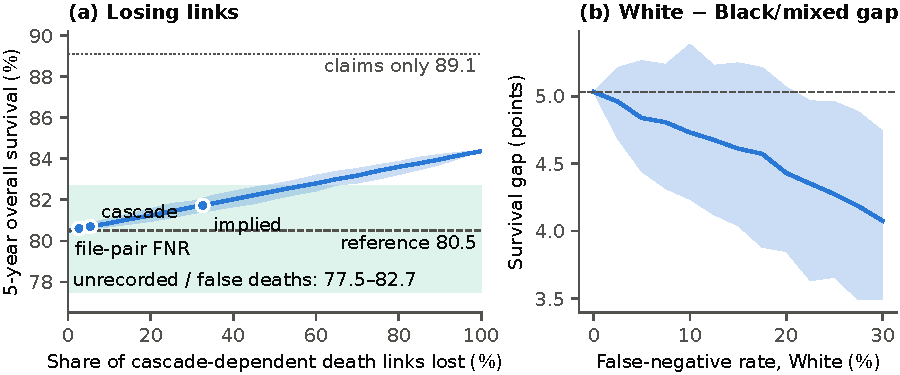
\includegraphics[width=\linewidth]{figures/figB_propagation.pdf}}
\end{figure*}

\begin{figure}[ht]
\floatconts
  {fig:km}
  {\caption{Overall survival when death sources are omitted. Every missed death
  becomes a censored patient, so survival is overstated from the first months.}}
  {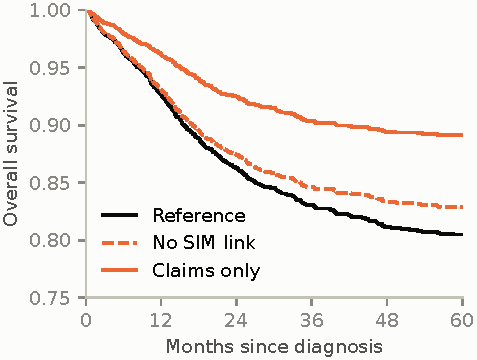
\includegraphics[width=\linewidth]{figures/figC_km_scenarios.pdf}}
\end{figure}

\subsection{Capture--Recapture and the Registry-Only Deaths}

\begin{table}[ht]
\floatconts
  {tab:decomp}
  {\caption{Registry-only deaths ($n$=111), searched in SIM by date of
  death + birth date. The same search finds 85\% of the deaths
  both sources hold.}}
  {\small
  \begin{tabular}{@{}L{0.8\linewidth}r@{}}
  \toprule
  Outcome of the search & $n$ \\
  \midrule
  In SIM; our link failed on the diagnosis-code filter & 16 \\
  In SIM; municipality of residence differs & 7 \\
  In SIM; passes all filters as reconstructed & 19 \\
  Not in SIM & 69 \\
  \quad after the key's miss rate (upper bound) & 61 \\
  \quad of all 111: entered by the municipality route & 5 \\
  \bottomrule
  \end{tabular}}
\end{table}

The two death lists overlap: 229 deaths in both, 111 only in
the registry, 134 only in the pipeline. Within five years the pipeline
also records 67.4\% [62.2, 72.1] of the registry's deaths; this is an overlap between two
incomplete lists, not a recall. The Chapman estimator
$\hat N=(n_1+1)(n_2+1)/(m+1)-1$ with Seber's variance gives 539
[515, 563] deaths; the pipeline captures 67\%, the
registry 63\% and their union 88\%; patients of unknown
stage are captured least (69\%). Stratified by stage, time to death
or year, the unrecorded deaths number 58--75;
they are added among survivors of each stage in proportion to the stratified
estimate. Dependence between lists (a well-registered patient appears in both)
would make $\hat N$ too small; false links in a list make it too large.

The direct search uses no municipality and no diagnosis code; it misses deaths
whose recorded dates disagree between sources, at a rate $b$ =
15\% among the deaths both lists hold. With $F$ false deaths among
the $N$ registry-only ones, the not-found count is $F + b(N-F)$, so
$F = (\text{not found} - bN)/(1-b)$ = 61. This is an upper bound: $b$
is measured on deaths the link had already found, which are easier to find than
a true death it missed. Without these likely false deaths, capture--recapture
estimates 29 unrecorded deaths instead of 65. The search key needs both dates to agree; among
children a coincidental death with the same birth and death date is negligible.

\subsection{The Registry Link}
\label{app:rhclink}
The registry link uses no birth date (the registry records age at diagnosis). It
was re-run inside SIA on 53,346 chemotherapy and radiotherapy records
(which carry a diagnosis date and the CNS) against patient identities: at the
75-day window it links 92.6\% of probes with precision 93.6\% and
recall 86.7\%. Because each probe also contributes to its reference
identity, these are upper bounds. The municipality fallback is unreliable
(0 of 119 correct). The 55 cohort patients
linked that way remain in the reference cohort; they account for
5 of the 111 registry-only deaths, and excluding them
gives OS 80.7\% and HR 2.56. Restricting to the strictest
matches (same hospital, diagnosis dates within 7 days, same estimated birth year;
$n$=785) gives OS 84.0\% [81.0, 86.5] and HR
3.12; across strict strata OS ranges
80.7--84.0\% and HR 2.56--5.16. The strict
OS lies above the bracket of Figure~\ref{fig:scenarios}, which is the direction
false registry deaths predict; strict matches may also select better-kept
records, so this is a subsample, not a correction.

\subsection{Race as the Missing Variable}
\label{app:race}
Of the 2{,}622 White, Black/mixed and race-missing patients, 119 lack race
(Table~\ref{tab:race}).

\begin{table}[ht]
\floatconts
  {tab:race}
  {\caption{White vs.\ Black/mixed-race patients, nephroblastoma cohort, with race
  as the missing variable. All three assume that race is missing at random given
  the covariates.}}
  {\small
  \begin{tabular}{@{}L{0.42\linewidth}rr@{}}
  \toprule
  Method & HR [95\% CI] & OS gap \\
  \midrule
  Complete case & 0.741 [0.610, 0.900] & 5.0 \\
  Inverse probability weighting & 0.743 [0.610, 0.904] & 5.2 \\
  Multiple imputation & 0.734 [0.604, 0.891] & 5.3 \\
  \bottomrule
  \end{tabular}}
\end{table}

Complete case: HR (White vs.\ Black/mixed) 0.741 [0.610, 0.900], OS gap 5.0 points.
Inverse probability weighting, with the probability that race is recorded
modelled on age, sex, stage, region, year, treatment group, the 5-year event and
the Nelson--Aalen cumulative hazard, stabilised by the marginal probability
(weights 0.96--1.52), robust variance: 0.743 [0.610, 0.904], gap
5.2. Multiple imputation (20 imputations, logistic imputation
model including the outcome, Rubin's rules \citep{rubin1987}): 0.734 [0.604, 0.891], gap
5.3. Inverse probability weighting and complete case agree because the
covariates predict missing race weakly; all three assume that race is missing at
random given the covariates.

\section{Breast-Cancer Model: Full Results}
\label{app:c50}

\begin{table}[ht]
\floatconts
  {tab:c50stage}
  {\caption{Crude mortality over follow-up (to December 2024) by stage under
  each label, breast-cancer model population.}}
  {\small
  \begin{tabular}{@{}l@{\hspace{4pt}}r@{\hspace{5pt}}r@{\hspace{5pt}}r@{}}
  \toprule
  & Pipeline & Registry & Union \\
  \midrule
  Stage I & 7.4\% & 11.4\% & 16.7\% \\
  Stage IV & 41.8\% & 24.4\% & 50.4\% \\
  Ratio IV/I & 5.7 & 2.1 & 3.0 \\
  \bottomrule
  \end{tabular}}
\end{table}

\runin{The pipeline label} Of its 40,755 deaths, 23,966
(59\%) are flags on the patient's own chemotherapy, radiotherapy or
hospital records (C1, no link, dated at the last record) and 16,789 come from
the SIM link (C2); the registry confirms 36\% and 26\%
of them. The stage IV/I mortality ratio is 7.5 for C1 and
3.9 for C2: deaths during treatment concentrate in advanced stage,
which steepens the pipeline gradient.

\runin{Registry-only deaths} They make up 9.3\% of stage I and
8.6\% of stage IV patients, whereas pipeline-only deaths rise from
5.3\% to 26.0\%. Searched in SIM by date of death and birth
date, 5,612 of 18,144 are found, against
69\% of deaths both sources hold; the key's hit rate itself rises
with stage (55\% in stage I, 73\% in stage
IV). Correcting for the key's miss rate as in Appendix~\ref{app:casestudy}
(overall, and stage by stage for the split), about 9,988 registry-only
deaths (55\%; 32\% of all
registry-labelled deaths) are not in SIM: 61\% in stage I
against 32\% in stage IV. In adults this figure is indicative
only: the key's hit rate is measured on deaths already linked (overstating it),
and a coincidental death with the same birth and death date is not rare
(understating it); the stage pattern is the robust part. Capture--recapture on
these lists would imply a 46\% mortality and is not usable here.

\runin{Calibration and injected loss} Within its own label each model is
calibrated (decile error 0.8, 0.6 and
1.1 points; Figure~\ref{fig:calib}); against the union, the
pipeline- and registry-trained models under-predict (predicted/observed
0.68 and 0.55). By race, against the union, the
pipeline model under-predicts White, mixed-race and Black patients by
9.6, 7.4 and 9.6 points; the
registry model by 9.7, 14.0 and
14.9. Under the registry label the region HRs are extreme (South
0.46, Southeast 1.87; pipeline 1.04,
1.40): registry death follow-up differs by hospital. We inject loss
into the 12,344 deaths that exist solely through the SIM link (C2, not in
the registry). Lost at the per-race file-pair FNR (about 462, 50 draws), the stage IV HR is
4.29 and the decile error 1.1 points; at the cascade's loss
(668 lost), 4.28; at five times the measured rate,
4.21 and 1.4.

\begin{figure}[ht]
\floatconts
  {fig:calib}
  {\caption{Calibration-in-the-large (predicted $-$ observed 5-year risk, test
  set) for each training label, evaluated on each label.}}
  {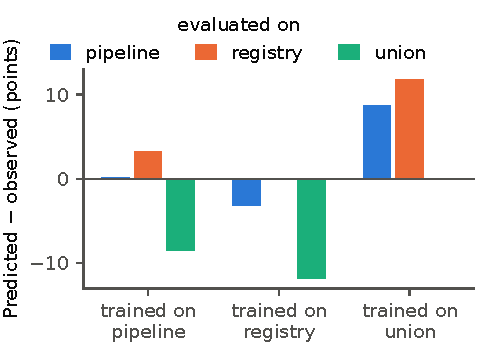
\includegraphics[width=\linewidth]{figures/figD_calibration.pdf}}
\end{figure}

\section{Reproducibility}
\label{app:repro}
Every number in this paper is read from an aggregate output table by a script
that maps it to its source cell, and every figure is drawn from the same tables.
The scripts, the aggregate tables and that map are in the repository given in the
Data and Code Availability statement, together with synthetic-data scripts that
reproduce the check-digit validation and the Fellegi--Sunter calculations.
Record-level files are not released.

\end{document}
